\section{Packages}

\begin{figure}[H]
    \centering
    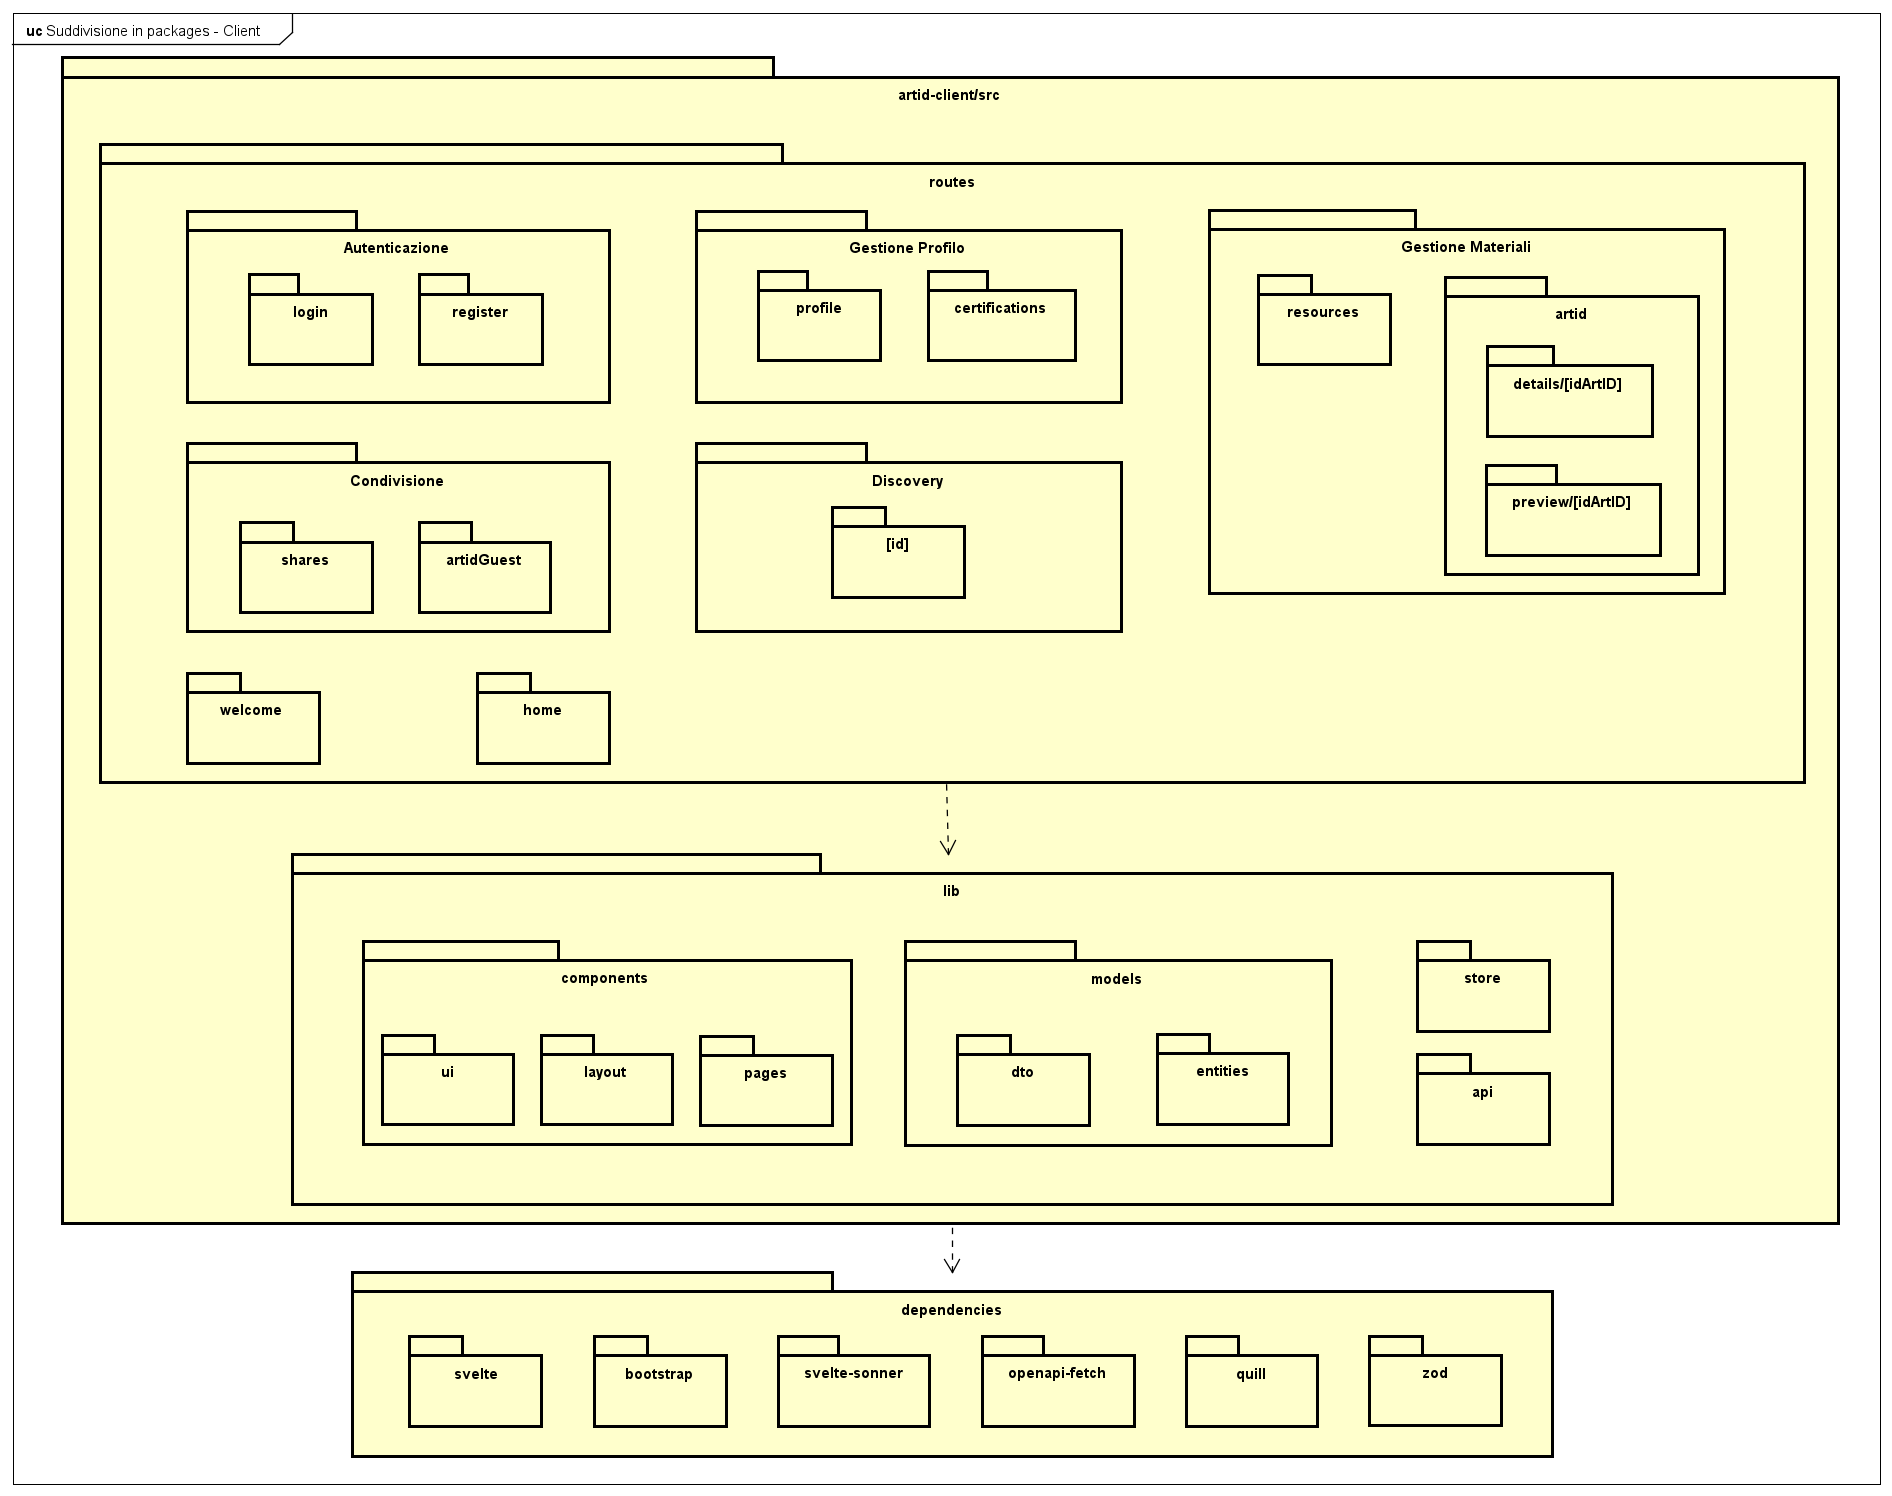
\includegraphics[width=0.95\textwidth, height=0.90\textheight, keepaspectratio]{Immagini/Suddivisione in packages - Client.png}
    \caption{Suddivisione in packages - Client}
\end{figure}

\begin{figure}[H]
    \centering
    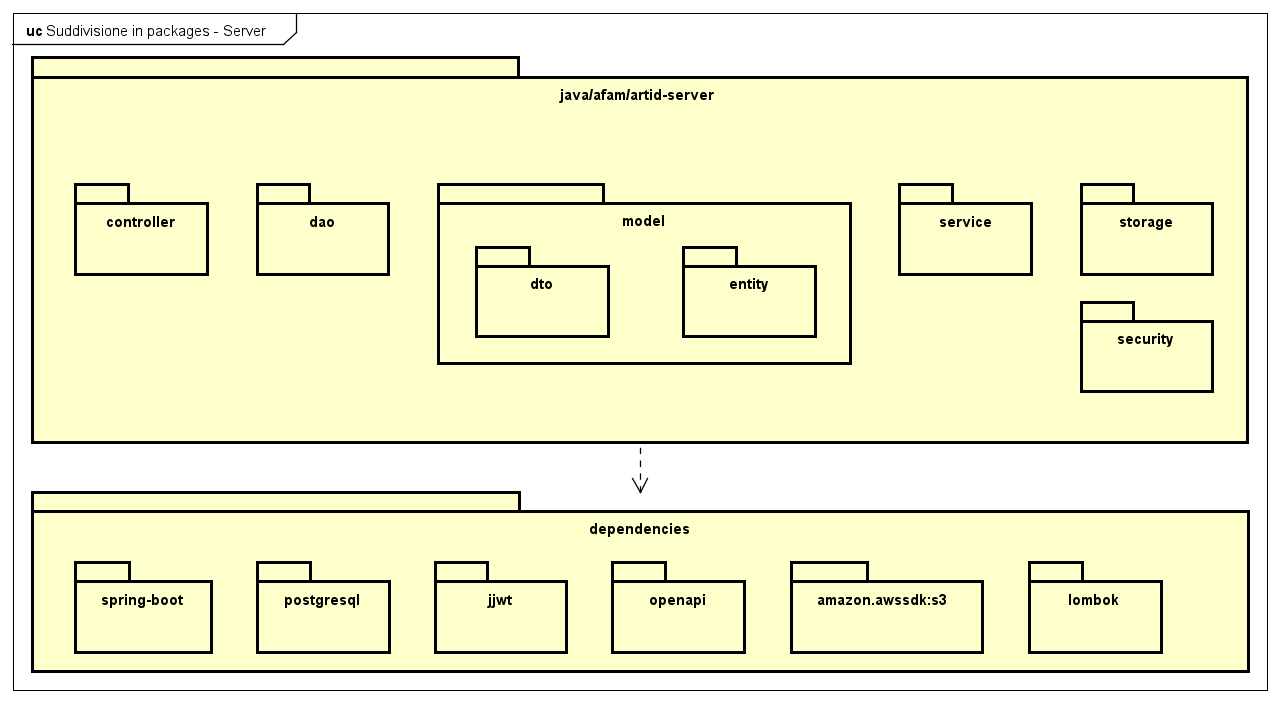
\includegraphics[width=0.95\textwidth, height=0.90\textheight, keepaspectratio]{Immagini/Suddivisione in packages - Server.png}
    \caption{Suddivisione in packages - Server}
\end{figure}

\clearpage

\subsection{\texttt{artid-client/src}}
Questa cartella contiene il \textbf{Front-end} dell'applicazione.\\
La struttura sfrutta il routing basato sul file system e la separazione netta tra l'interfaccia grafica e la logica di caricamento dati.

\subsubsection{\texttt{routes}}
Questa cartella definisce l'albero dei \textbf{percorsi navigabili} dell'applicazione; secondo le convenzioni di SvelteKit, ad ogni sottocartella corrisponde un URL accessibile dal browser.

Al fine di mantenere la coerenza con i requisiti del RAD e i diagrammi dell'SDD, è stato introdotto un layer di cartelle fittizie che non alterano il routing, ma servono a raggruppare logicamente i percorsi in base ai relativi macro-casi d'uso.

Il \textbf{punto di accesso} principale all'applicazione è definito nella cartella:
\begin{itemize}
    \item \texttt{welcome}: contiene il file \texttt{+page.svelte} che implementa la GUI della Landing Page e fornisce i controlli di navigazione iniziali verso le sezioni di autenticazione.
\end{itemize}
La pagina principale dopo l'autenticazione si trova nella cartella:
\begin{itemize}
    \item \texttt{home}: contiene il file \texttt{+page.svelte} che implementa l'interfaccia di controllo centrale, esponendo i collegamenti rapidi a tutte le sezioni funzionali dell'applicazione.
\end{itemize}

Di seguito vengono dettagliati i percorsi raggruppati per macro-casi d'uso:

\paragraph{Autenticazione}
Area dedicata alla gestione dell'accesso e dell'identità:
\begin{itemize}
    \item \texttt{login}: composta da \texttt{+page.svelte} per la GUI del form e \texttt{+page.server.ts} per la gestione sicura delle richieste di accesso lato server e l'integrazione con lo \textbf{SPID}.
    \item \texttt{register}: composta da \texttt{+page.svelte} (interfaccia di registrazione) e \texttt{+page.server.ts} (validazione e invio dei dati di iscrizione al back-end).
\end{itemize}

\paragraph{Gestione Profilo}
Area che permette al Membro di amministrare le proprie informazioni personali:
\begin{itemize}
    \item \texttt{profile}: formata da \texttt{+page.svelte} e \texttt{+page.server.ts}; consente la modifica dei dati del Membro, il cambio password, il collegamento dello \textbf{SPID} e la disattivazione dell'account.
    \item \texttt{certifications}: formata da \texttt{+page.svelte} e \texttt{+page.server.ts}; fornisce gli strumenti per il caricamento, la visualizzazione e la gestione delle certificazioni professionali del Membro.
\end{itemize}

\paragraph{Gestione Materiali}
Area fulcro dell'applicazione per la manipolazione degli asset digitali:
\begin{itemize}
    \item \texttt{resources}: formata da \texttt{+page.svelte} e \texttt{+page.server.ts}; permette la gestione CRUD (caricamento, rimozione, download e modifica) dei Materiali del Membro.
    \item \texttt{artid}: formata da \texttt{+page.svelte} e \texttt{+page.server.ts}; dedicata alla creazione guidata e alla consultazione dell'elenco dei propri \texttt{ArtID}.
    \item \texttt{artid/details/[idArtID]}: percorso dinamico formato da \texttt{+page.svelte} e \texttt{+page.server.ts} per l'ispezione approfondita e la consultazione dei metadati di uno specifico \textbf{ArtID}.
    \item \texttt{artid/preview/[idArtID]}: percorso dinamico formato da \texttt{+page.svelte} e \texttt{+page.server.ts} che genera un'anteprima dell'\textbf{ArtID}.
\end{itemize}

\paragraph{Condivisione}
Sezione predisposta per la condivisione degli \textbf{ArtID}:
\begin{itemize}
    \item \texttt{shares}: formata da \texttt{+page.svelte} e \texttt{+page.server.ts}; permette al Membro di monitorare, revocare o generare nuovi link.
    \item \texttt{artIDGuest}: formata da \texttt{+page.svelte} e \texttt{+page.server.ts}; rappresenta la vista pubblica o ad accesso limitato dedicata ai soggetti esterni che consultano un \textbf{ArtID} condiviso.
\end{itemize}

\paragraph{Discovery}
Sezione pubblica per la ricerca dei Membri:
\begin{itemize}
    \item \texttt{explore}: formata da \texttt{+page.svelte} e \texttt{+page.server.ts}; implementa i filtri e il motore di ricerca globale per trovare i profili dei Membri all'interno della piattaforma.
    \item \texttt{explore/[id]}: percorso dinamico formato da \texttt{+page.svelte} e \texttt{+page.server.ts}; permette la visualizzazione in sola lettura del profilo pubblico di un Membro selezionato.
\end{itemize}

\subsubsection{\texttt{lib}}
Questa cartella agisce da contenitore per tutte le risorse condivise, le logiche riutilizzabili e i moduli trasversali dell'applicazione Front-end. Al suo interno risiedono anche i modelli TypeScript speculari a quelli definiti nel server Java.

\paragraph{\texttt{components}}
Raccolta dei componenti dell'interfaccia utente, organizzati secondo principi di riusabilità:
\begin{itemize}
    \item \texttt{layout}: contiene i componenti macroscopici e strutturali dell'applicazione, come la barra di navigazione globale \texttt{artid-navbar.svelte}.
    \item \texttt{pages}: ospita componenti complessi dedicati a specifiche schermate, isolati per alleggerire il codice dei file \texttt{+page.svelte} principali.
    \item \texttt{ui}: collezione di componenti atomici e privi di stato (stateless), riutilizzabili in qualsiasi sezione del software, come il pulsante stilizzato \texttt{artid-button.svelte}.
\end{itemize}

\paragraph{\texttt{models}}
Gestisce la controparte client delle strutture dati del database:
\begin{itemize}
    \item \texttt{dto}: definisce le interfacce TypeScript che ricalcano l'esatto formato dei messaggi scambiati tramite chiamate \textbf{API REST} con il \textbf{back-end}.
    \item \texttt{entities}: definisce i modelli ad oggetti in ambiente TypeScript (\texttt{.ts}) che rappresentano la struttura logica delle entità memorizzate nel sistema.
\end{itemize}

\paragraph{\texttt{stores}}
Questa cartella si occupa della gestione dello stato globale dell'applicazione.\\ Centralizza le informazioni accessibili da più componenti:
\begin{itemize}
    \item \texttt{auth.ts}: mantiene in memoria l'istanza e i dettagli del Membro correntemente autenticato, esponendo i metodi globali per verificare i permessi di sessione e lo stato dell'autenticazione in tempo reale.
\end{itemize}

\paragraph{\texttt{api}}
Centralizza la definizione dei contratti di interfaccia e i meccanismi di comunicazione diretta con il \textbf{Back-end}, implementando un approccio basato su \textbf{API-First Design}:
\begin{itemize}
    \item \texttt{schema.d.ts}: file di definizione dei tipi TypeScript generato automaticamente a partire dal file di specifica tramite appositi tool di compilazione; mappa rigorosamente i modelli del database e le risposte del server, azzerando il rischio di disallineamento dei dati e garantendo il controllo statico dei tipi in tutto il Front-end.
\end{itemize}

\subsection{\texttt{java/afam/artid-server}}
Questo package costituisce il nucleo del \textbf{Back-end} dell'applicazione, suddiviso nelle seguenti componenti.

\subsubsection{\texttt{controller}}
Questa cartella contiene i componenti \textbf{REST Controller} responsabili di esporre gli endpoint \textbf{API} verso il \textbf{Front-end}. Il loro compito principale è intercettare le richieste HTTP, validare i dati in ingresso e delegare l'esecuzione della logica di business al rispettivo \texttt{service}. Inoltre, i \textbf{Controller} si occupano di mappare e convertire i risultati ricevuti dal service nei relativi \texttt{dto} (Data Transfer Object) prima di impacchettare e restituire la risposta HTTP al front-end.

\subsubsection{\texttt{dao}}
Contiene le interfacce \textbf{DAO} (Data Access Object) responsabili dell'interazione diretta con il database relazionale. Sfruttando le specifiche di \textbf{Spring Data JDBC} tramite l'estensione di \texttt{ListCrudRepository}, è sufficiente dichiarare il prototipo del metodo nella firma dell'interfaccia per demandare al framework la generazione automatica della query SQL a runtime. Tuttavia, per operazioni complesse o manipolazioni custom, il sistema consente la scrittura di query personalizzate sfruttando l'annotazione \texttt{@Query}.

\subsubsection{\texttt{model}}
Questo package definisce le strutture dati utilizzate all'interno dell'applicazione ed è suddiviso in due sottopackage principali:

\paragraph{\texttt{dto}}
Contiene i \textbf{Data Transfer Object} (\texttt{DTO}), ovvero classi Java fittizie utilizzate esclusivamente per \textbf{modellare} e \textbf{standardizzare} il formato dei messaggi e dei payload scambiati nelle richieste e risposte HTTP tra il front-end e il back-end.

\paragraph{entity}
Contiene le classi Java che rappresentano l'esatta mappatura delle tabelle presenti nel Database. Queste classi sono modellate secondo i requisiti di \textbf{Spring Data JDBC} (utilizzando le annotazioni del pacchetto \texttt{org.springframework.data.relational.core.mapping}) e sfruttano la libreria \texttt{Lombok} (che tramite l'annotazione \texttt{@Data} genera automaticamente a tempo di compilazione tutti i metodi getter, setter, costruttori e codice boilerplate equivalente) per massimizzare la leggibilità del codice.

\subsubsection{\texttt{service}}
Questa cartella contiene le classi in cui è implementata la \textbf{logica di business} dell'applicazione. I componenti di questa cartella orchestrano il flusso dei dati interni: ricevono gli input dai \texttt{controller}, interrogano o modificano lo stato del database invocando i relativi \texttt{dao}, applicano le regole applicative e i controlli di consistenza, e infine restituiscono gli oggetti di business o le entità elaborate direttamente ai \texttt{controller}.

\subsubsection{\texttt{storage}}
Questo package gestisce la persistenza degli asset digitali (Materiali, allegati e foto profilo) sfruttando un'infrastruttura di Object Storage esterna. Contiene le classi di configurazione e i servizi per l'interazione con endpoint S3-compatibili.

\subsubsection{\texttt{security}}
Questo package centralizza l'intera infrastruttura di autenticazione e controllo degli accessi dell'applicativo basata su \textbf{Spring Security}. Configurato in modalità rigorosamente \textbf{stateless} tramite l'utilizzo di token \textbf{JWT}, gestisce il ciclo di vita delle sessioni utente senza sovraccaricare il server. 

Al suo interno risiedono le componenti per la generazione e validazione crittografica dei token JWT, il filtro per l'intercettazione e il controllo delle richieste HTTP, la configurazione della catena di sicurezza con la definizione dei permessi delle rotte.